\documentclass[conference]{IEEEtran}
\IEEEoverridecommandlockouts
% The preceding line is only needed to identify funding in the first footnote. If that is unneeded, please comment it out.
\usepackage{cite}
\usepackage{amsmath,amssymb,amsfonts}
 \usepackage[ruled,vlined]{algorithm2e}
\usepackage{graphicx}
\usepackage{textcomp}
\usepackage{xcolor}
\usepackage{float}
\usepackage{tikz}
\usetikzlibrary{arrows.meta}
\def\BibTeX{{\rm B\kern-.05em{\sc i\kern-.025em b}\kern-.08em
    T\kern-.1667em\lower.7ex\hbox{E}\kern-.125emX}}
\begin{document}

\title{Distributed Forecasting Framework for Energy Consumption\\
}

\author{\IEEEauthorblockN{1\textsuperscript{st} Simion Oltean}
\IEEEauthorblockA{\textit{Department of Computer Science} \\
\textit{ Technical University of Cluj-Napoca}\\
Cluj-Napoca, Romania \\
Oltean.Se.Simion@student.utcluj.ro}
\and
\IEEEauthorblockN{2\textsuperscript{nd} Marcel Antal}
\IEEEauthorblockA{\textit{Department of Computer Science} \\
\textit{Technical University of Cluj-Napoca}\\
Cluj-Napoca, Romania \\
Marcel.Antal@campus.utcluj.ro}
}

\maketitle
\begin{abstract}
This paper explores the task of forecasting electricity consumption per hour in buildings using a time series approach. In this study, we design a distributed time series forecasting framework for ASHRAE's G.E.P. III competition dataset, involving cloud-based data acquisition, leakage-safe features extraction, autocorrelated lag-24 building selection, and strictly chronological validation. The study compares performance of Random Forest, Support Vector Regression, and XGBoost models versus daily persistence and weekly same-hour mean baselines in the context of this distributed pipeline. Empirical evaluations on three ASHRAE buildings prove that the global Random Forest attains the most accurate performance overall: MAE 16.758 and $R^2=0.8388$ in the autumn setting, and MAE 13.749 and $R^2=0.9403$ in the winter setting. In comparison to the best classical baseline in each case, this amounts to MAE improvements of 68.3\% and 71.9\%, correspondingly. Season-filtering has been found to be overall inferior in prediction accuracy.
\end{abstract}
\begin{IEEEkeywords}
building energy forecasting, electricity consumption, time-series validation,
machine learning, ASHRAE G.E.P. III, Random Forest, seasonal training, feature
importance
\end{IEEEkeywords}
\raggedbottom
\begin{figure*}[t]
\centering
\includegraphics[width=0.8\textwidth]{pipeline.jpg}
\caption{Overview of the data acquisition, preprocessing, model training, and forecasting stages in a building energy prediction pipeline.}
\label{fig:related-work-forecasting-context}
\end{figure*}
\section{Introduction}

The research is conducted in the scope of smart grid energy system applications, focusing more precisely on the application to electricity demand prediction at building level. Buildings are considered one of the major consumers of electricity, and electricity consumption at buildings is a process that depends on a schedule, weather conditions, building operation, and seasonality aspects. In turn, the problem discussed here is that of forecasting hourly electricity consumption, where the information used for predictions is time-dependent, contains missing values, and differs across buildings. The problem is thus formulated as the inability to predict hourly electricity consumption in buildings, and to do so in a way to retain predictions consistent with real-world data over time after forecasting is performed. Evaluation metrics are chosen as RMSE, MAE, nMAE, and $R^2$ – that is, they reflect absolute prediction error, scale-dependent prediction error, and prediction variance, respectively.

The discussed problems are tackled in this paper by applying our approach of forecasting time-aware workflows to the ASHRAE GEPIII 2019 dataset. Our starting point is meter readings, meteorological information, and building meta-data that we use to produce hourly time series for further supervised regression modeling. One of the crucial aspects here is that we make no use of any future information during transition from initial dataset to prepared-for-modeling data. This means that we need to consider both handling missing data and feature engineering, all based on past data. Additionally, the current research uses lag-24 autocorrelation to choose representative buildings.

The objective of the paper is to design, and implement a distributed framework for ML predictive techniques in order to forecast the hourly electrical consumption demand of the selected buildings. The predictive algorithms considered are random forest, support vector regression, and extreme gradient boosting, while daily persistence and weekly same hour mean will be used as benchmarks. In addition to comparing the performance of various predictive algorithms, the paper also tries to examine if the seasonal filtering technique is more efficient in training than the global chronological technique for the same test dataset. The issue is significant because the seasonal technique could be more accurate since it is specialized but uses lesser samples during training. Variable and group-wise permutation importance measures are used to identify the most influential features.

The remainder of this paper is organized as follows. The work done in the
area of building energy consumption forecast, seasonal modeling, and
prediction using machine learning techniques is highlighted in
Section~\ref{sec:related-work}. In Section~\ref{sec:proposed-solution}, we
discuss our proposed approach that covers preprocessing, feature
construction, representative buildings' selection, model training, and
validation method. The experiments conducted on the ASHRAE GEPIII 2019
dataset are presented in Section~\ref{sec:experiments-validation}. The section~\ref{sec:conclusion} concludes the paper and summarizes the current limitations
and future directions.




\section{Related Work}
\label{sec:related-work}

In this section, the background research required to solve the problem will be presented.
Topics that will be covered include forecasting of building energy, load prediction with machine learning, preprocessing of data and seasonality, and where this work fits into energy prediction.


\subsection{Building Energy Consumption Forecasting}

A variety of machine learning techniques are employed in constructing an
energy prediction model because electrical demand is determined by non-linear
relationships involving weather conditions, scheduling, building use, and past
consumption. Random Forest technique has proven to be useful in predicting
hourly building energy usage, compared to individual regression trees and
Support Vector Regression algorithms using building data \cite{Wang2018RFHourly}.
The study is important in this paper for two reasons: firstly, it emphasizes the
robustness of tree ensemble algorithms relative to individual trees. Secondly, it
proves that seasonality or semester division of data can influence prediction.
Other studies have utilized statistical and machine learning approaches for
determining building energy efficiency \cite{Tsanas2012EnergyBuild}.

Ensemble algorithms play a particularly crucial role in such applications since
simple learning algorithms may easily overfit noisy information from buildings.
The authors, Wang et al., used ensemble bagging trees to estimate building
energy use, arguing that using multiple tree-based models outperforms a single
CART-like model in terms of robustness \cite{Wang2018EnsembleLearning}.
Feature importance based on permutations is also highlighted in the same work,
which can be useful in cases where the task requires predicting consumption
and determining the sets of features that affect the prediction. Ensemble-based
prediction techniques have also been explored in studies concerning the
prediction of next-day building energy consumption and peak demands,
suggesting that hybridized models may offer better prediction results for
commercial buildings \cite{Fan2014NextDayBuildingEnergy}. Such literature
inspires the application of Random Forest and XGBoost in this paper, since both
are ensemble decision trees capable of modeling non-linear relationships in the
absence of explicit equations.

\subsection{Kernel Models, Preprocessing, and Seasonality}

Another promising field for further analysis may become a study on the usage of SVM and SVR algorithms for energy forecasting. The authors of \cite{Shao2020HotelSVM} have applied SVM algorithm for forecasting hotel buildings' energy consumption and reached decent performance, which was possible thanks to the preprocessing of data and their parameters tuning. This is because the energy consumption in hotel buildings is rather nonlinear with respect to HVAC and human behavior, just as in institutional buildings. There are also works devoted to electricity consumption forecasting using SVM models, which are capable of competing with regression and ANN models, provided that proper scaling is done \cite{Kaytez2015ForecastingElectricity}. That is why, applying SVR after scaling is crucial.

Moreover, from reviewing related literature, one can understand that data preprocessing, quality, and validation technique play a key role in model performance. Specifically, it is known that data obtained from energy measurements in buildings include holes and oddities, thus applying any occupancy proxy techniques is not feasible. Therefore, it is important to deal with the way data can be concatenated, processed, partitioned, and validated. Additionally, an important aspect is related to the seasonality, which is because models that are trained on larger time windows have certain peculiarities in contrast to models trained on the same season. This research follows this idea by comparing global training and season-based training on the same validation time.

\subsection{Broader Energy Context and System Boundary}

Other research papers in the domain of the smart grid are concerned with predicting renewable energy generation and implementing non-intrusive load monitoring. The findings of the studies concerned with the prediction of the generation of renewable energy suggest that a machine learning approach is applicable if the dependent variable is nonlinearly related to the meteorological factors and time \cite{Rahman2021HRESANN}. Other researchers use fuzzy or grey methods for predicting renewable generation, which again implies the significance of considering seasonality and nonlinearity \cite{Cao2021RT3FLS,Qian2021SADGM}. While these papers deal with energy generation, not consumption in buildings, they confirm the same main idea.

Non-Intrusive Load Monitoring (NILM) is a concept that bears some relation to energy disaggregation but deals with a distinct problem. In NILM, the goal is the decomposition of aggregate electrical consumption in terms of appliance consumption via one or several meters \cite{Zoha2012NILMSurvey}. This study does not involve the disaggregation of consumption to the appliance level. It involves forecasting the meter reading for a building at the point of time in the future. This distinction is key because it accounts for why the voltage/current signal is not considered here. Rather, the relevant data points are lagged consumption, rolling statistics, meteorological readings, calendar variables, and building attributes. Relative to previous research, this paper's innovation is not in the algorithm, but in the end-to-end workflow including pre-processing, model selection, baseline comparison, validation, and interpretation of results.

Considering all the related work presented, our approach aims to offer: 
\begin{itemize}
    \item \textbf{I}:  A complete \textit{distributed forecasting framework} that incorporates the elements most relevant to the identified problem.
    \item \textbf{II}: A construction of relevant time dependent \textit{features} for ensemble and kernel-based regression.
    \item \textbf{III}: \textit{Seasonal} versus \textit{global regime} evaluation and model interpretation.
\end{itemize}



Based on the literature review of all the relevant studies conducted, the method that will be proposed in this paper can be considered to be an example of a reproducible hourly electricity forecasting process. In other words, there will be no invention of a brand-new prediction algorithm, but rather an integration of all previously developed approaches.


\section{Models and Algorithms}
\label{sec:proposed-solution}
This section outlines the forecast algorithm pipeline that was suggested.
It details the mathematical model of the forecast problem,
the constructed features groups, the representatives selection algorithm,
and the services implementation of the pipeline.


The solution approach includes an end-to-end forecasting pipeline that converts the ASHRAE GEPIII 2019 dataset into supervised learning tasks, selects relevant buildings, trains the baseline and non-baseline models, and evaluates global versus seasonal training using chronological validation. This solution comprises two parts. 

\begin{figure}[H]
\centering
\resizebox{\columnwidth}{!}{
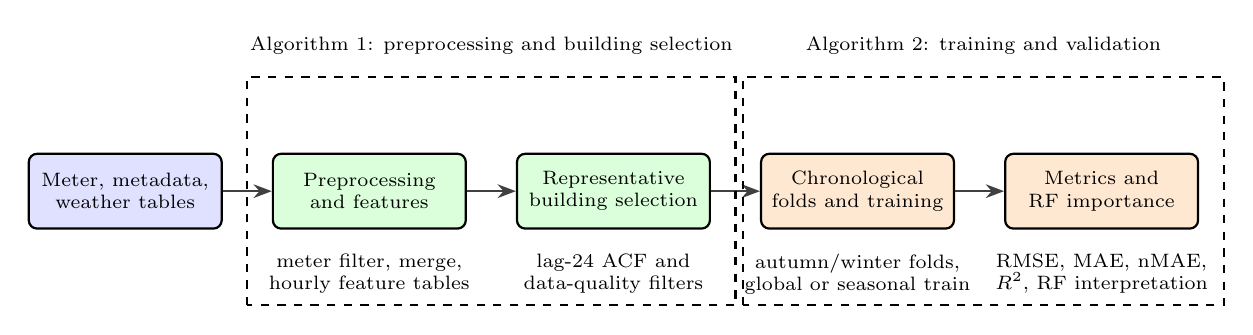
\begin{tikzpicture}[
    >=Stealth,
    stage/.style={
        draw,
        rounded corners=3pt,
        thick,
        align=center,
        minimum width=2.45cm,
        minimum height=0.95cm,
        font=\scriptsize
    },
    flow/.style={->, thick, draw=black!75},
    note/.style={font=\scriptsize, align=center}
]

\node[stage, fill=blue!12] (data) at (0,0) {Meter, metadata,\\weather tables};
\node[stage, fill=green!14] (features) at (3.1,0) {Preprocessing\\and features};
\node[stage, fill=green!14] (selection) at (6.2,0) {Representative\\building selection};
\node[stage, fill=orange!18] (models) at (9.3,0) {Chronological\\folds and training};
\node[stage, fill=orange!18] (eval) at (12.4,0) {Metrics and\\RF importance};

\draw[flow] (data) -- (features);
\draw[flow] (features) -- (selection);
\draw[flow] (selection) -- (models);
\draw[flow] (models) -- (eval);

\draw[dashed, thick] (1.55,-1.45) rectangle (7.75,1.45);
\draw[dashed, thick] (7.85,-1.45) rectangle (13.95,1.45);

\node[note] at (4.65,1.85) {Algorithm 1: preprocessing and building selection};
\node[note] at (10.9,1.85) {Algorithm 2: training and validation};

\node[note] at (3.1,-1.05) {meter filter, merge,\\hourly feature tables};
\node[note] at (6.2,-1.05) {lag-24 ACF and\\data-quality filters};
\node[note] at (9.3,-1.05) {autumn/winter folds,\\global or seasonal train};
\node[note] at (12.4,-1.05) {RMSE, MAE, nMAE,\\$R^2$, RF interpretation};

\end{tikzpicture}
}
\caption{Algorithm-level structure of the proposed forecasting solution.}
\label{fig:paper-solution-approach}
\end{figure}


Figure~\ref{fig:paper-solution-approach} shows how the two algorithms organize the forecasting workflow. The first part starts from the meter, metadata, and weather tables, then produces hourly feature tables and applies lag-24 autocorrelation and data-quality filters to select representative buildings. The second part uses the selected buildings to construct chronological autumn and winter folds, train the global or seasonal models, and report the metrics and Random Forest interpretation results.

\subsection{Mathematical Models}

Hourly electrical consumption is considered to be a time series regression problem.
For each building at time $t$, the forecast for the upcoming meter reading is given by the formula:
\begin{equation}
    \hat{y}_t = f(\mathbf{x}_t),
    \label{eq:forecasting-formulation-paper}
\end{equation}
Here, $\mathbf{x}_t$ includes all information known at or prior to the time of prediction. This data comprises a concatenation of past load values, calendar variables, weather data, building properties, and non-linear transformations. The key lags include:
\begin{equation}
    \ell_t^{(1)} = y_{t-1}, \qquad \ell_t^{(24)} = y_{t-24}.
\end{equation}
The former represents short-term inertia, whereas the latter reflects periodic daily building behavior.

Recent consumption statistics and volatility are represented using rolling
statistics on delayed load measurements, which avoids future leakage:
\begin{equation}
    \mu_t^{(w)} = \frac{1}{w}\sum_{i=1}^{w} y_{t-i},
\end{equation}
\begin{equation}
    \sigma_t^{(w)} =
    \sqrt{\frac{1}{w-1}\sum_{i=1}^{w}\left(y_{t-i}-\mu_t^{(w)}\right)^2}.
\end{equation}
The methodology utilizes rolling periods of 24 hours and 168 hours. Calendar
features are captured by the hour, day-of-week, month, day-of-month,
weekend, and business-hour dummies. Periodicity in the hour feature is coded as:
\begin{equation}
    s_t^{(h)} = \sin\left(\frac{2\pi h_t}{24}\right), \qquad
    c_t^{(h)} = \cos\left(\frac{2\pi h_t}{24}\right).
\end{equation}
Weather variables are comprised of: air temperature, dew point temperature,
cloud cover, precipitation amount, sea level pressure, wind direction, and
wind speed. A nonlinear interaction between hour and temperature is also
included:
\begin{equation}
    x_t^{(h,T)} = h_t T_t.
\end{equation}

The daily repetition of the load is also used for building selection through the
sample autocorrelation function:
\begin{equation}
    r_k = \frac{c_k}{c_0}, \qquad
    c_k = \frac{1}{T}\sum_{t=k+1}^{T}(y_t-\bar{y})(y_{t-k}-\bar{y}).
\end{equation}
In this paper, $r_{24}$ indicates the association between the corresponding hours of
consecutive days. This index is applied to select representative buildings with
enough internal structure of their daily profiles to make an interesting forecasting test.
\subsection{Algorithms}

The primary sequence of algorithms is split into two succinct phases, as described in Figure~\ref{fig:paper-solution-approach}.


\begin{algorithm}[H]
\scriptsize
\DontPrintSemicolon
\caption{Preprocessing and building selection}
\label{alg:prep-selection-paper}
\KwIn{Meter, metadata, and weather tables}
\KwOut{\texttt{per\_building}, \texttt{final\_buildings}}
$train \leftarrow$ rows from meter table where \texttt{meter = 0}\;
Add missingness indicators to metadata; median-fill numeric metadata\;
One-hot encode \texttt{primary\_use}; keep metadata for buildings in $train$\;
Keep weather rows for selected site ids; merge train, metadata, and weather tables\;
\ForEach{building $b$ in merged table}{
    $df \leftarrow$ rows of $b$ sorted by timestamp\;
    Add hour, weekday, month, day, weekend, and business-hour variables\;
    Resample $df$ to hourly frequency; Forward/backward fill static \texttt{primary\_use} columns\;
    Forward-fill \texttt{meter\_reading} with limit 24; drop missing target rows\;
    Interpolate weather columns with bounded limit, then forward/backward fill\;
    Add \texttt{load\_lag\_1h}, \texttt{load\_lag\_24h} and shifted 24h and 168h rolling mean and standard deviation\;
    Add \texttt{hour\_x\_temp}, \texttt{hour\_sin}, and \texttt{hour\_cos}\;
    \texttt{per\_building[$b$]} $\leftarrow df$ after dropping remaining invalid rows\;
}
\ForEach{building $b$}{
    Assign $b$ to its active \texttt{primary\_use} category\;
    Restrict $b$ to months 1--6 and compute lag-24 autocorrelation $r_{24}(b)$\;
}
\ForEach{primary-use category $c$}{
    Select representative closest to the median $r_{24}$ of category $c$\;
}
Rank category representatives by distance to global median $r_{24}$\;
Keep top candidates with max gap $<7$ days, missing ratio $<0.1$, and duration $\ge310$ days\;
\Return \texttt{per\_building}, selected category--building pairs\;
\end{algorithm}

Algorithm ~\ref{alg:training-paper} explains the process for validation and model comparison.
Chronological folds are created every month after an initial training
phase. Two folds are used: one with an autumn fold where November is
the test month, and the other with a winter fold where December is
the test month.


\begin{algorithm}[H]
\scriptsize
\DontPrintSemicolon
\caption{Chronological training and evaluation}
\label{alg:training-paper}
\KwIn{Selected buildings, engineered data, model set $M$}
\KwOut{Metrics, predictions, and Random Forest importances}
\ForEach{selected building $b$}{
    Sort engineered dataframe chronologically\;
    Build monthly expanding windows starting after the first 8 months\;
    Retain the fold whose validation month is November as autumn, and the fold whose validation month is December as winter\;
    \ForEach{fold $f \in \{\textnormal{autumn},\textnormal{winter}\}$}{
        $test \leftarrow$ fixed validation month of $f$\;
        $train \leftarrow$ all data before $test$\;
        \ForEach{strategy $s \in \{\textnormal{global},\textnormal{seasonal}\}$}{
            \If{$s$ is seasonal}{
                Filter $train$ to the season months of $f$\;
            }
            Split $train$ and $test$ into $X$, $y$ by removing \texttt{meter\_reading}\;
            \ForEach{model $m \in M$}{
                Resolve cached grid for $(m,s,b,f)$ or fit with \texttt{TimeSeriesSplit}\;
                Predict on the unchanged validation window\;
                Compute RMSE, MAE, nMAE, and $R^2$\;
            }
        }
    }
}
For Random Forest, compute feature importance and grouped permutation importance\;
\end{algorithm}


The three learning algorithms that will be compared in this comparison include the Random Forest Algorithm, the Support Vector Regression Algorithm, and the XGBoost algorithm. The algorithms are compared with respect to daily persistence,
$\hat{y}_t=y_{t-24}$, and weekly same-hour averaging,
$\hat{y}_t=\frac{1}{7}\sum_{j=1}^{7}y_{t-24j}$. 


The three regression models are complementary because they operate on different principles of regression. In the case of the Random Forest Model, the predictions from $B$ regression trees are averaged:
\begin{equation}
    \hat{f}_{RF}(x) = \frac{1}{B}\sum_{b=1}^{B}T_b(x).
\end{equation}
Each tree partitions the predictor space into regions and assigns a constant
prediction to each region:
\begin{equation}
    f(x)=\sum_{m=1}^{M}c_m I(x \in R_m), \qquad
    \hat{c}_m=\frac{1}{|R_m|}\sum_{x_i\in R_m}y_i.
\end{equation}

\begin{figure}[H]
\centering
\includegraphics[width=\columnwidth]{dt_regions.png}
\caption{Regression-tree partitioning used as the base mechanism for
tree-ensemble forecasting models.}
\label{fig:paper-dt-regions}
\end{figure}

For Support Vector Regression, the model balances flatness and fitting error
through the regularized $\varepsilon$-insensitive objective:
\begin{equation}
    \min_{w,b}\frac{1}{2}\lVert w\rVert^2
    + C\sum_{t=1}^{n}(\xi_t+\xi_t^*).
\end{equation}
After introducing Lagrange multipliers, the prediction function can be written
in kernel form as:
\begin{equation}
    f(x)=\sum_{n=1}^{N}(a_n-\hat{a}_n)K(x_n,x)+b.
\end{equation}
In the implemented SVR model, nonlinearity is represented through the RBF
kernel:
\begin{equation}
    K(x_i,x_j)=\exp(-\gamma \lVert x_i-x_j\rVert^2).
\end{equation}
For XGBoost, the boosted tree is fitted using gradient information from the loss function. 
With a second-order approximation, the local contribution of an update $\gamma$ can be
expressed as:
\begin{equation}
    L(y_i,\hat{y}_i+\gamma)\approx
    L(y_i,\hat{y}_i)+g_i\gamma+\frac{1}{2}h_i\gamma^2,
\end{equation}
where $g_i$ and $h_i$ are the first and second derivatives of the loss with
respect to the current prediction. For a terminal region $R_{jm}$, the optimal
output value used by the tree is:
\begin{equation}
    \gamma_{jm} =
    -\frac{\sum_{x_i\in R_{jm}} g_i}
    {\sum_{x_i\in R_{jm}} h_i+\lambda}.
\end{equation}
These equations relate the models developed to the theory proposed in this thesis:
tree partitioning, similarity using kernels, additive boosting, and regularized trees
trained by gradients. The resulting equation is:
\begin{equation}
    f_m(x) = f_{m-1}(x) + \sum_{j=1}^{J_m} \gamma_{jm} \mathbf{1}(x \in R_{jm})
\end{equation}


\subsection{Distributed Data-Framework Architecture}



The implementation is based on a containerized microservices architecture:

\begin{figure}[H]

\centering
\includegraphics[width=0.4\textwidth]{deployment.pdf}
\caption{System deployment diagram.}
\label{fig:system-deployment}
\small
\end{figure}


The \textit{data-cloud} microservice deals with storing and retrieving the ASHRAE datasets and grid-search artifact in Cloudflare R2. Also, it performs conversions from local CSV files to Parquet in case of necessity and exposes endpoints for uploading the dataset and grid-search artifact. The \textit{data-preprocess} microservice downloads the Parquet dataset from \textit{data-cloud}, merges all the required tables, generates engineered dataframe per each building, computes lag-24 autocorrelation, selects the final buildings list and creates visualization for preprocessing procedure. \textit{Model-training} microservice requests selected buildings list from \textit{data-preprocess}, performs the chronological split of train/test datasets, trains the baseline and ML models, calculates the performance metric, makes predictions and prediction plots, and returns the Random Forest feature importance values.


The client interacts with the system via a  frontend application interface. The frontend
starts the preprocessing pipeline and invokes endpoints for the models and shows
the status information about stages of execution, graphs, metrics, prediction
plots and feature importances calculation results. The entire project is developed using
Docker Compose with different services which provide access to the cloud storage with the data, preprocess, train the models and provide the frontend.


\section{Experiments and Validation}
\label{sec:experiments-validation}

The following analysis describes how the suggested predictive system will be tested on the representative buildings. This testing will also follow the stated purposes mentioned before, such as evaluating the appropriateness of developed predictors for predictions, comparison of the global and season-based training, and possibility to interpret the Random Forest model by using feature importance.

\subsection{Experimental Setup}

The experimental datasets are drawn from the ASHRAE Great Energy Predictor
III 2019. The source tables are merged into a single source. As the paper
only concentrates on predicting electricity usage, only the data rows concerning electricity consumption are kept. After the merging of tables,
weather readings, and building metadata, the preprocessing component works with
about 12 million rows and 32 columns, generating hourly series for 1,400
buildings.

The final testing step is conducted on three representative buildings chosen by
the method outlined in Section~\ref{sec:proposed-solution}. These buildings are
listed in Table~\ref{tab:selected-buildings-paper}. Each selected building
includes roughly 8,500--8,600 hourly data points, and their acf values are around 0.72--0.74.

\begin{table}[H]
\centering
\caption{Representative buildings used in validation.}
\label{tab:selected-buildings-paper}
\begin{tabular}{lc}
\hline
\textbf{Primary-use category} & \textbf{Building id} \\
\hline
Healthcare & 1209 \\
Education & 1088 \\
Public services & 460 \\
\hline
\end{tabular}
\end{table}

These are the metrics used to evaluate the models: RMSE, MAE, normalized MAE, and $R^2$. The methodology for running the experiments includes the preprocessing step followed by the execution of the endpoints for training the models, including both the baselines and the non-baselines. The two folds of validation chosen for each experiment are the "autumn" one, where the test is performed in November, and the "winter" one, where the test is conducted in December.

\begin{table}[H]
\centering
\scriptsize
\caption{Compared forecasting methods and tuning settings.}
\label{tab:model-config-paper}
\begin{tabular}{p{0.27\linewidth}p{0.63\linewidth}}
\hline
\textbf{Method} & \textbf{Configuration} \\
\hline
Random Forest & Trees $\in \{100,200\}$; min leaf samples $\in \{10,15\}$;  \\
SVR & \texttt{StandardScaler()} followed by RBF-kernel SVR; $C$ and $\varepsilon$ derived from the training-target standard deviation; $\gamma \in \{\texttt{scale},0.001,0.01\}$. \\
XGBoost & Trees $\in \{100,500,1000\}$; depth $\in \{3,6\}$; learning rate $\in \{0.05,0.1\}$; subsample and column-sample values $\in \{0.8,1.0\}$. \\
\hline
\end{tabular}
\end{table}

The comparison considers two classical benchmarks and three machine learning regressors. Table~\ref{tab:model-config-paper} shows the predictive techniques and their hyperparameters used in the paper. The benchmarks give straightforward time-dependent comparisons, whereas the machine learning algorithms are optimized using time series cross-validation to prevent using future observations in training.


For all non-baseline models, hyperparameters are selected using
GridSearchCV with TimeSeriesSplit. A fixed random seed of 42 is used for stochastic
tree-based models.

\subsection{Experimental Results}

Results have been divided into sections according to the validation cases. Considering that there are three example buildings in each case, Tables~\ref{tab:autumn-results-paper} and~\ref{tab:winter-results-paper} give the average measures for the chosen buildings.

\begin{table}[H]
\centering
\scriptsize
\caption{Average performance in the autumn scenario.}
\label{tab:autumn-results-paper}
\begin{tabular}{llcccc}
\hline
\textbf{Model} & \textbf{Mode} & \textbf{RMSE} & \textbf{MAE} & \textbf{nMAE} & \textbf{$R^2$} \\
\hline
Random Forest & Global & 48.999 & 16.758 & 0.0303 & 0.8388 \\
Random Forest & Seasonal & 51.828 & 20.049 & 0.0414 & 0.7984 \\
SVR & Global & 55.905 & 26.906 & 0.0409 & 0.7736 \\
SVR & Seasonal & 56.048 & 28.302 & 0.0412 & 0.7678 \\
XGBoost & Global & 49.674 & 19.648 & 0.0361 & 0.8278 \\
XGBoost & Seasonal & 50.425 & 21.198 & 0.0436 & 0.8003 \\
Naive & Seasonal & 97.517 & 54.431 & 0.0762 & 0.2187 \\
Weekly mean & Seasonal & 79.326 & 52.811 & 0.0828 & 0.4507 \\
\hline
\end{tabular}
\end{table}

\begin{table}[H]
\centering
\scriptsize
\caption{Average performance in the winter scenario.}
\label{tab:winter-results-paper}
\begin{tabular}{llcccc}
\hline
\textbf{Model} & \textbf{Mode} & \textbf{RMSE} & \textbf{MAE} & \textbf{nMAE} & \textbf{$R^2$} \\
\hline
Random Forest & Global & 23.682 & 13.749 & 0.0242 & 0.9403 \\
Random Forest & Seasonal & 54.742 & 33.269 & 0.0310 & 0.8762 \\
SVR & Global & 39.392 & 30.067 & 0.0394 & 0.8758 \\
SVR & Seasonal & 81.495 & 59.376 & 0.0728 & 0.6350 \\
XGBoost & Global & 25.741 & 16.513 & 0.0317 & 0.9225 \\
XGBoost & Seasonal & 56.993 & 34.981 & 0.0320 & 0.8684 \\
Naive & Seasonal & 78.903 & 48.984 & 0.0711 & 0.4469 \\
Weekly mean & Seasonal & 89.271 & 69.106 & 0.0853 & 0.4617 \\
\hline
\end{tabular}
\end{table}

The optimal averages are achieved by the Global Random Forest in both situations with an error of 16.758 and $R^2=0.8388$ in the fall season and 13.749 and $R^2=0.9403$ in the winter season. As compared to the best baseline in each scenario, this implies a reduction of MAE by 68.3\% in the fall and 71.9\% in the winter seasons. The seasonal approach to training is not uniformly beneficial either, although it can help in individual cases like the winter case of Building 460.

Per-building best configurations are consistent with the mean values as well. The Global Random Forest model is the best for all autumn buildings and the Healthcare 1209 and Education 1088 buildings during winter. The only exception is the Public services 460 building during winter, when the seasonal Random Forest model yields the lowest MAE. It shows that the seasonal approach may be helpful at the building level under some circumstances.

The importance scores from the random forest algorithm confirm the choice of features. Table~\ref{tab:feature-importance-paper} highlights the most powerful individual features and the grouped permutation importance. It can be seen that the history of loads is the key feature, while cyclical time data are secondary. Weather and metadata features have relatively insignificant influence on the prediction accuracy.

\begin{table}[H]
\centering
\scriptsize
\caption{Random Forest feature-importance summary.}
\label{tab:feature-importance-paper}
\begin{tabular}{p{0.24\linewidth}p{0.42\linewidth}p{0.24\linewidth}}
\hline
\textbf{Analysis} & \textbf{Feature or group} & \textbf{Value} \\
\hline
Individual effect & load\_lag\_1h& 0.9190 \\
Individual effect & hour\_cos& 0.0348 \\
Individual effect & hour& 0.0157 \\
Individual effect & hour\_sin& 0.0085 \\
Individual effect & load\_lag\_24h& 0.0072 \\
Group  effect & Lag features & MAE +4.89 \\
Group  effect & Nonlinear features & MAE +0.79 \\
Group  effect & Time features & MAE +0.25 \\
\hline
\end{tabular}
\end{table}


\section{Conclusion}
\label{sec:conclusion}

In this paper, a distributed, time-aware forecasting framework was provided for the prediction of building electricity consumption on an hourly basis based on the ASHRAE GEPIII 2019 dataset. All the tasks defined within the scope of the paper were carried out. In this regard, the task of data preparation and preprocessing was fulfilled via combining metering data, weather conditions, and building-related features in order to build feature tables at the building level based on historical data. Time-aware evaluation was achieved through chronological folds ensuring the preservation of the order of the data as well as the same months for validation between global and seasonal training models. All of this is done using separate modular microservices with docker containerization.

The results from the experiment indicate that the constructed feature set is adequate for accurate prediction of the selected buildings. The selected buildings exhibit high regularity within a day, as demonstrated in Fig.~\ref{fig:paper-validation-acf}.

\begin{figure}[H]
\centering
\includegraphics[width=\columnwidth]{validation_acf_selected.png}
\caption{Lag-24 autocorrelation values for the representative buildings used in
validation.}
\label{fig:paper-validation-acf}
\end{figure}

It can be seen from Tables~\ref{tab:autumn-results-paper} and~\ref{tab:winter-results-paper}
that learning-based models exhibit better performance than their daily persistence
and weekly same-hour mean counterparts, with the  exception of SVR in the winter scenario, with a seasonal configuration. This can be explained by the fact that the steep drops and irregularities do affect the possibility of SVR finding a suitable kernel to capture that behavior. The best-performing model configuration,
the global Random Forest, achieves a mean absolute error (MAE) of 16.758 and
$R^2 = 0.8388$ for the autumn case and an MAE of 13.749 and $R^2 = 0.9403$
for the winter case. In comparison with the best-performing classical model,
the relative MAE improvement is 68.

\begin{figure}[H]
\centering
\includegraphics[width=\columnwidth]{validation_mae_comparison.png}
\caption{Average MAE comparison across models, training modes, and validation
scenarios.}
\label{fig:paper-validation-mae}
\end{figure}

The forecast trace in Fig.~\ref{fig:paper-rf-1209-winter} shows that the global
Random Forest follows the observed winter consumption pattern for Building 1209.

\begin{figure}[H]
\centering
\includegraphics[width=\columnwidth]{validation_rf_1209_winter_global.png}
\caption{Predicted versus actual electricity consumption for Building 1209
using the global Random Forest model in the winter scenario.}
\label{fig:paper-rf-1209-winter}
\end{figure}

The Random Forest importance results also support the design of the feature set,
since recent load, daily lag, and cyclical hour information are the main
predictive factors.

The contrast between global and seasonal training showed that the hypothesis
regarding improved accuracy due to seasonal filtering cannot be considered
to have satisfied the initial hypothesis. In spite of the theoretical foundation of the seasonal approach,
it should be used on an individual basis since the lesser number of training
samples usually leads to the increased stability of the global chronological
method. The limitations of the research are connected with the fact that the
validation involved only three buildings rather than the entire population
used by ASHRAE, that only autumn and winter scenarios were chosen, and that
the interpretability aspect was analyzed only based on Random Forest method.
Further papers may involve the validation for other buildings and seasons,
as well as further exploration of interpretation tools.



\bibliographystyle{IEEEtran}
\bibliography{thesis}


\end{document}
